\section{Complex Examples}

\subsection{Mathematics}

\begin{frame}{Mathematical Foundations}
    \begin{pblock}{Euler's Identity}
        \[ e^{i\pi} + 1 = 0 \]
    \end{pblock}
    
    \begin{palert}{Schrödinger Equation}
        \[ i\hbar \frac{\partial}{\partial t} \Psi(\mathbf{r},t) = \left [ \frac{-\hbar^2}{2m}\nabla^2 + V(\mathbf{r},t) \right ] \Psi(\mathbf{r},t) \]
    \end{palert}
    
    Matrix operations:
    \[
    \begin{pmatrix}
        a & b \\
        c & d
    \end{pmatrix}
    \times
    \begin{pmatrix}
        x \\
        y
    \end{pmatrix}
    =
    \begin{pmatrix}
        ax + by \\
        cx + dy
    \end{pmatrix}
    \]
\end{frame}

\subsection{TiKZ Diagram}

\begin{frame}{Deep Learning Architecture (TiKZ)}
    \centering
    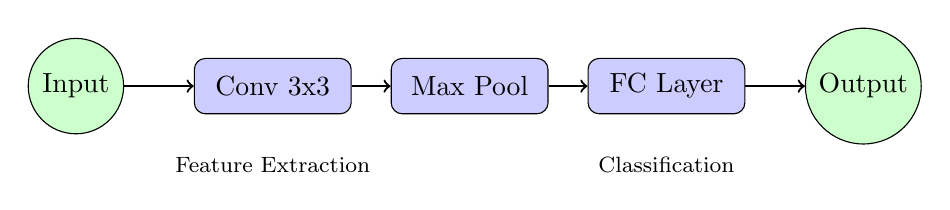
\begin{tikzpicture}[node distance=1.5cm, auto]
        \tikzstyle{layer} = [rectangle, draw, fill=blue!20, text width=5em, text centered, rounded corners, minimum height=2em]
        \tikzstyle{data} = [circle, draw, fill=green!20, text centered, minimum size=2em]
        
        \node [data] (input) {Input};
        \node [layer, right of=input, xshift=1cm] (conv1) {Conv 3x3};
        \node [layer, right of=conv1, xshift=1cm] (pool1) {Max Pool};
        \node [layer, right of=pool1, xshift=1cm] (fc1) {FC Layer};
        \node [data, right of=fc1, xshift=1cm] (output) {Output};
        
        \draw [->, thick] (input) -- (conv1);
        \draw [->, thick] (conv1) -- (pool1);
        \draw [->, thick] (pool1) -- (fc1);
        \draw [->, thick] (fc1) -- (output);
        
        \node[below of=conv1, yshift=0.5cm] {\footnotesize Feature Extraction};
        \node[below of=fc1, yshift=0.5cm] {\footnotesize Classification};
    \end{tikzpicture}
\end{frame}

\subsection{Algorithms}

\begin{frame}{Algorithm Implementation}
    \begin{algorithm}[H]
        \SetAlgoLined
        \KwData{Input image $I$}
        \KwResult{Normalized image $I'$}
        $min, max \gets \text{compute\_range}(I)$\;
        \For{each pixel $p \in I$}{
            $I'(p) \gets \frac{I(p) - min}{max - min} \times 255$\;
        }
        \caption{Min-Max Normalization}
    \end{algorithm}
\end{frame}

\subsection{Layouts}

\begin{frame}[fragile]{Split Layout Examples}
    \begin{columns}[T] % [T] aligns columns at the top
        \begin{column}{0.48\textwidth}
            \begin{pblock}{Left Column (Blocks)}
                Standard 50/50 split using:
                \begin{itemize}
                    \item \texttt{columns} environment
                    \item \texttt{column} environment
                \end{itemize}
                This is great for comparing text with images or code.
            \end{pblock}
        \end{column}
        
        \begin{column}{0.48\textwidth}
            \begin{pinfo}{Right Column (Info)}
                You can place anything here:
                \begin{itemize}
                    \item Tables
                    \item Graphics
                    \item Equations
                \end{itemize}
            \end{pinfo}
        \end{column}
    \end{columns}
\end{frame}

\begin{frame}[fragile]{Asymmetric Split (60/40)}
    \begin{columns}[c] % [c] aligns columns vertically at the center
        \begin{column}{0.6\textwidth}
            \begin{pycode}[title=Processing Logic]
def analyze_data(data):
    # Complex math here
    result = [x**2 for x in data]
    return sum(result)
            \end{pycode}
        \end{column}
        
        \begin{column}{0.35\textwidth}
            \begin{palert}{Observation}
                The left column takes 60\% width for code, while this alert takes 35\% for explanation.
            \end{palert}
        \end{column}
    \end{columns}
\end{frame}

\subsection{Code Snippets}

\begin{frame}[fragile]{Source Code (C++ \& Python)}
    \begin{columns}
        \begin{column}{0.5\textwidth}
            \begin{codeblock}[title=main.cpp]{C++}
#include <iostream>

int main() {
    // Hello Panda!
    std::cout << "Hi!" << std::endl;
    return 0;
}
            \end{codeblock}
        \end{column}
        \begin{column}{0.5\textwidth}
            \begin{pycode}[caption=Python Snippet]
import numpy as np

def hello():
    print("Hello from Python!")
    return np.zeros(5)
            \end{pycode}
        \end{column}
    \end{columns}
\end{frame}
